\section{Approaches for Further Improvements}\label{sec:resolution}
As already discussed, the percentage of defined translations is small. Therefore, extending the backend libraries with additional translations for more semantic macros is the first obvious task to improve the translator. Adding more \gls{cas} would also be worthwhile for forward and backward translations. Some \gls{cas} or other software use other notations than the infix notations. Therefore, another improvement for the translator would be the support for other types of notations. This could be achieved by using expression trees during the translation process rather than the \gls{mlp-pt} generated by the \gls{mlp}.

Another minor issue is the way of representing functions after a backward translation. The \Macro s allow different representations and control the different styles by the number of $@$ symbols. Currently the backward translation simply adds the largest possible number of $@$ symbols, which has undesirable effects. Categorizing the functions (Possible categories may be \textit{trigonometric functions} or \textbf{polynomials}) can be used to define the right typical number of $@$ symbols for the most common representations.

Besides the extensions for the backend libraries, we saw in \cref{sec:numerical-tests} that automatic numerical tests are not implemented yet. Certainly, automatic numerical tests are a powerful approach to verify translations and also to find errors in the mathematical sources. However, the realization of such powerful numerical tests is very difficult. As far as we know, there is no general theory for such methods developed yet. An approach could be to adapt error handling methods in telecommunications such as the cyclic redundancy checks~\cite{CRC} that use checksums to detect errors. Adapting such approaches for general mathematical functions could be helpful.

The most desirable improvement for the translator is the support for generic \LaTeX. Since the semantic \LaTeX{} macros are newly invented and generic \LaTeX{} is still the de facto standard for mathematical expressions, it is definitely worthwhile to support generic \LaTeX{} later on. However, we already explained the difficulties of this task. One approach we want to realize is the \textbf{multiple-scan approach}. This approach is inspired by the approach of humans. When a human reader reads mathematical expressions, he concludes the correct semantics from the structure and the context of the expression. His conclusions highly depend on his own knowledge. If he is not familiar with a mathematical symbol, he has difficulties to understand the whole expression.

The multiple-scan approach tries to adapt these techniques with the following three objectives:
\begin{enumerate}[label=(\arabic*)]
\item\label{multi-scan-1} narrow down possible meanings only from the expression itself, without referring to the context of the expression;
\item\label{multi-scan-2} refine the process with conclusions from the nearby context of the expressions and
\item\label{multi-scan-3} improve the previous process by analyzing not only the nearby context but the overall topic of the whole scientific paper or book, its references and other publications by the authors.
\end{enumerate}
Starting with the lexicon files from the \gls{pom}-tagger, we want to narrow down the possible meanings of an expression. It is planned to extend the \gls{pom}-tagger from \cite{POM-Tagger} to achieve objective~\ref{multi-scan-1}. Furthermore, a large-scale corpus study has shown that around 70 percent of the symbolic elements in scientific papers are denoted in the surrounded text \cite{SymbolDec}. With this awareness we can achieve objective~\ref{multi-scan-2} by just searching the close context \cite{MLP:Project,SIGIR:Semantification,MORITZ:Evaluating}. If the correct semantic information is still unsure, objective~\ref{multi-scan-3} is the last way to find a solution. Online compendia, such as arXiv, can be used to discover the overall topic of a scientific paper, the references and the area of research of the authors. The MCAT search engine developed by Kristianto, Topic and Aizawa \cite{MCAT,MCAT:MathSemanticSearch} is able to extract and score information from the document at this '\textit{document granularity level}'. Ideally, there is only one possible interpretation left after step~\ref{multi-scan-3}. Otherwise, even a human reader might have difficulties to understand the expression.

Figure~\ref{fig:multiple-scan} visualizes the process of conclusions for the Jacobi polynomial example from \cref{tab:JacobiP-usecase}.

\begin{figure}[htp]
	\centering
	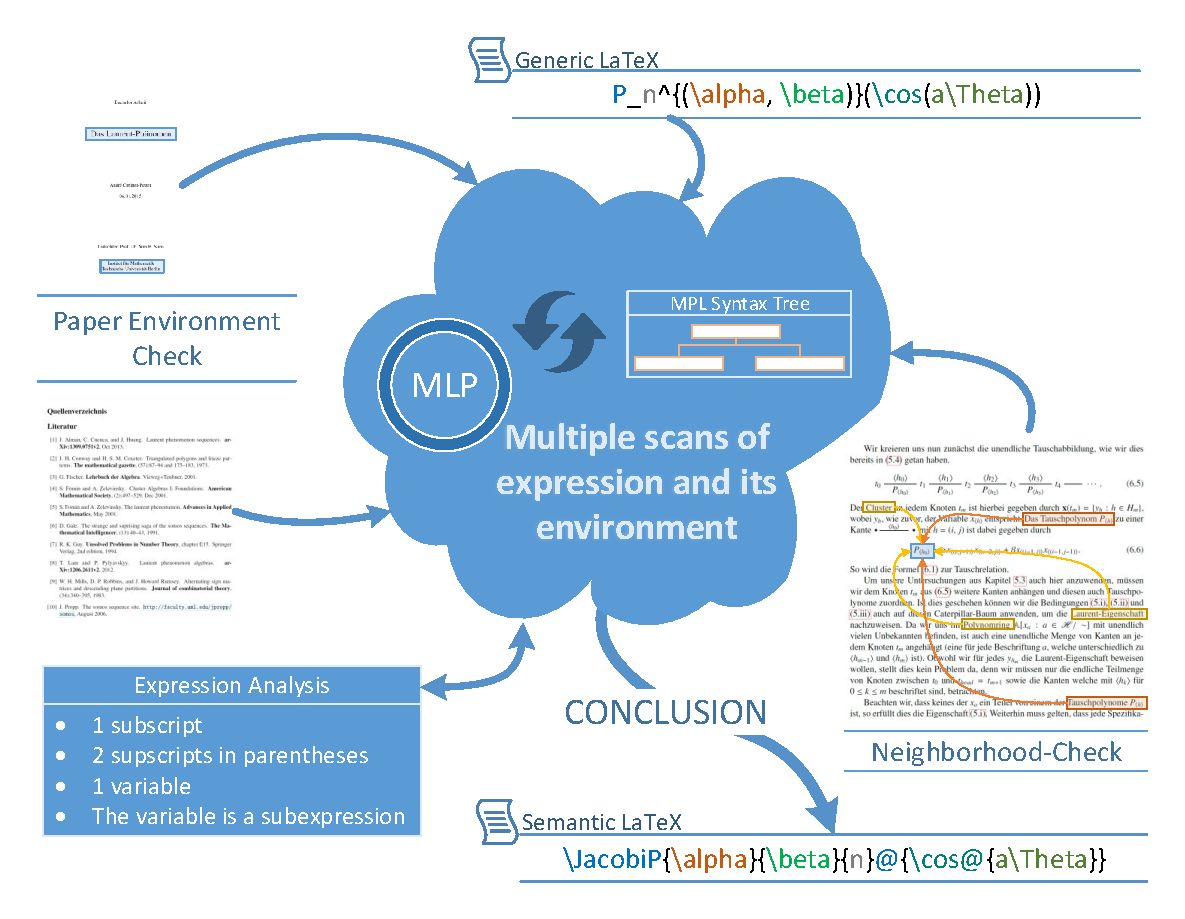
\includegraphics[clip, trim=0.1cm 0.1cm 0.1cm 0.1cm, scale=0.7]{MultipleScanApproach.pdf}
	\caption{Visualization of the multiple-scan approach. Exemplified using the Jacobi polynomial example.}
	\label{fig:multiple-scan}
\end{figure}

With such improvements the translator possibly becomes multifunctional: from automatic translations between word processors and computer algebra systems over to a verification tool for mathematical compendia, then over to a tool that can automatically enrich mathematical expressions with semantic information. A combination of the automatic semantically enrichment process and \LaTeX{} extraction tools~\cite{MaxTract} would be even hypothetically able to semantically enrich already published articles in PDF format afterwards.

\cleardoublepage